\documentclass{article}
\usepackage[utf8]{inputenc}
\usepackage[T1]{fontenc}
\usepackage[german]{babel}
\usepackage{amsmath}
\usepackage{amsthm}
\usepackage{amsfonts}
\usepackage{amssymb}
\usepackage{minted}
\usepackage{tikz}
\usepackage{pgfplots}
\usepackage[top=2cm, bottom=2cm, left=2cm, right=2cm, headheight=1.5cm]{geometry}
\usepackage{fancyhdr}
\usepackage{mdframed}
\usemintedstyle{emacs}

\definecolor{purp}{HTML}{9A72AC}
\definecolor{re}{HTML}{FC6255}
\definecolor{gre}{HTML}{83C167}
\definecolor{blu}{HTML}{58C4DD}
\definecolor{shadecolor}{rgb}{0.85,0.85,0.85}
\definecolor{bg}{rgb}{0.95,0.95,0.95}
\setlength{\parindent}{0em} 

\BeforeBeginEnvironment{minted}{\begin{mdframed}[linewidth =2 ,backgroundcolor=bg , linecolor=black, linewidth=0.5]}
\AfterEndEnvironment{minted}{\end{mdframed}}

\newenvironment{defi}[1]{
    \begin{shaded*}
    \textbf{Definition #1} \\
}{
    \end{shaded*}
}

\newcommand{\bsp}{\textbf{Beispiel}:}
%\newcommand{\task}{\textbf{Aufgabe}:}

\newcommand{\bol}[1]{\textbf{#1}}
\newcommand{\q}[1]{\glqq #1\grqq}
\newcommand{\DODO}[1]{\textbf{\textcolor{red}{DODO:}} #1 \\ \begin{center}\includegraphics[scale=0.2]{../../media/dodo.jpg} \end{center}}

\newenvironment{task}[1]{
    \begin{shaded*}
    \textbf{Aufgabe #1}:
}{
    \end{shaded*}
}



\fancypagestyle{firstpage}{
    \setlength{\headheight}{2.5cm}
    \setlength{\footskip}{0.25cm}
    \pagestyle{fancy}
    \renewcommand{\headrulewidth}{0.4pt}
    \fancyhf{}
    \fancyhead[L]{\LARGE\textbf{Musterlösung und Erläuterungen S. 205|4}}
    \fancyfoot[C]{\thepage}
}
\begin{document}
\thispagestyle{firstpage}
\setlength{\headsep}{12pt}
\textbf{Hinweis:} Diese Musterlösung enthält nicht nur einen möglichen Lösungsquelltext, sondern versucht auch Gedankenprozesse, die während der Lösung der Aufgabe so auftreten könnten nachzubilden, d.h. die zuerst geschriebenen Code-Schnippsel sind noch nicht zwingend das Endergebnis, sondern möglicherweise Zwischenschritte. Alle Methoden befinden sich in einer Klasse, z.B. \textit{Würfeln}.
\vspace{0.5cm}
\textbf{Analyse der Aufgabe:} Liest man sich die Aufgabe durch, wird sofort klar, dass die in Teilaufgabe a) zu programmierende Würfelfunktion auch in der zweiten Teilaufgabe verwendet wird. Es bietet sich also an, eine eigene Methode mit Signatur \textit{public int würfeln()} zu definieren, die eine Zufallszahl zwischen 1 und 6 zurückgibt. \\
Ein erster Ansatz:
\begin{minted}{Java}
    public int würfeln() {
        int zufallszahl = Math.random()*6;
        return zufallszahl;
    }
\end{minted}
Man stellt schnell fest, dass Java hier nicht mitspielt. \textit{Math.random()} erzeugt zwar eine Zufallszahl, allerdings einen double zwischen 0 und 1 (ausgeschlossen). Das bedeutet, man muss den Bereich künstlich erweitern, z.B. indem man mit 6 multipliziert. Jetzt hat man allerdings noch das Problem, dass die zurückzugebende Zufallszahl ein Integer sein soll (das wird besonders für b) nützlich sein und entspricht auch mehr dem, was wir erwarten würden!. \\
Um das Problem zu lösen kann die Math.round() Funktion verwendet werden:
\begin{minted}{Java}
    public int würfeln() {
        int zufallszahl = Math.round(Math.random()*6);
        return zufallszahl;
    }
\end{minted}
Lässt man das Ganze so stehen, dann liefert Java aber immer noch einen Fehler \q{Incompatible types: possible lossy conversion from long to int}. \\
Eine kurze Suche fördert zu Tage, dass die round()-Funktion einen $long$ zurückgibt. Das ist ein Datentyp, der eine Ganzzahl beschreibt, die aber größer als ein $int$ sein kann. Java ist deswegen besorgt, dass das Ganze schief gehen könnte, nett! \\
Wir sind uns aber sicher, dass das hier keine Probleme macht, deswegen können wir einen sogenannten $cast$ verwenden, im Wesentlichen sagen wir dem Java-Compiler damit, dass wir uns hier sicher sind, dass es nur so groß wird wie ein Integer sein kann (wenn wir uns irren sind wir dann halt selber schuld..). Der folgende Code behebt die Fehlermeldung auf eigene Gefahr:
\begin{minted}{Java}
    public int würfeln() {
         return (int) Math.round(Math.random()*6);
    }
\end{minted}
Gleichzeitig habe ich noch eine kosmetische Veränderung vorgenommen: wenn wir nur etwas berechnen und in einer Zeile in eine Variable speichern und diese danach zurückgeben, können wir auch direkt den Wert berechnen und zurückgeben. 
\vspace{0.5cm}
Für Teilaufgabe b) sind doch einige Vorüberlegungen notwendig:
\begin{itemize}
    \item Wie im Unterricht bereits besprochen gibt es zwei Möglichkeiten die Würfelergebnisse zu speichern, in einem langen Array oder in einem kurzen Array der Länge 6, in dem wir nur die Anzahl der jeweils gewürfelten Zahl speichern (wer ein Bild vor Augen braucht: im zweiten Fall entspricht unser Array einer Reihe von 6 Eimern und jedes Mal wenn wir eine Zahl ziehen schmeißen wir sie in einen entsprechenden Eimer, z.B.: wir ziehen eine 1 $\Rightarrow$ ab in den ersten Eimer, etc. Am Ende zählen wir dann, wie viele Steine in den entsprechenden Eimern sind für die relative Häufigkeit.)
    \item Wir sollen 100, 1000 und 10000 mal würfeln. Wir könnten natürlich für alle drei Methoden schreiben, aber diese Methoden werden alle das GLeiche tun, nur mit einer unterschiedlichen Wiederholungsanzahl! Wir können also geschickter arbeiten, indem wir eine einzige Methode mit Eingabeparameter schreiben, die uns die Wiederholungsanzahl steuert!
    \item Zu Testzwecken bietet es sich an, das Array mit den Anzahlen manchmal auszugeben, damit wir nicht jedes mal for(...) schreiben müssen, können wir uns eine Methode \textit{ausgeben(int[] array)} definieren, die als Eingabeparameter ein Array mit Integers bekommt und dieses geeignet auf die Konsole ausgibt.
\end{itemize}
Mit diesen Vorüberlegungen wagen wir uns an die Aufgabe, wir definieren zuerst unsere Hilfsmethode:
\begin{minted}{Java}
    private void ausgeben(int[] array) {
        System.out.println();
        System.out.println("Das Array hat folgende Einträge: ");
        for(int i = 0; i < array.length; i++) {
            System.out.print(array[i] + " ");
        }
        System.out.println();
    }
\end{minted}
Die Methode kann private sein, da wir sie nur zu Hilfszwecken verwenden wollen. Wir laufen das Array durch und geben jeweils an der Stelle $i$ den Arrayeintrag mit \textit{array[i]} aus und fügen noch ein Leerzeichen an, da wir keinen Zeilenumbruch in der Ausgabe fordern (print statt println!). Am Anfang und am Ende fügen wir noch eine Leerzeile ein, damit es keine Konflikte mit eventuellen anderen Ausgaben gibt. Auf gehts zu unserer eigentlichen Methode:
\begin{minted}{Java}
    public void mehrfachWürfeln(int anzahl) {
        int[] ergebnisse = new int[6];
        for(int i = 1; i <= anzahl; i++) {
            //...
        }
    }
\end{minted}
Wir geben eine Zahl in unsere Methode ein und sagen damit, wie oft wir würfeln wollen. Diese Information verarbeiten wir in unserer Wiederholung. Wir beginnen bei $1$ zu zählen bis einschließlich \textit{anzahl}. Jetzt müssen wir uns überlegen, was wir 100 mal machen wollen: würfeln und Steine in Eimer schmeißen! Das geht so:
\begin{minted}{Java}
    public void mehrfachWürfeln(int anzahl) {
        int[] ergebnisse = new int[6];
        for(int i = 1; i <= anzahl; i++) {
            int gewürfelt = würfeln();
            ergebnisse[gewürfelt - 1] = ergebnisse[gewürfelt - 1] + 1;
        }
    }
\end{minted}
Wir würfeln einmal mit unserer in a) geschriebenen Methode und speichern das Ergebnis in der Variable gewürfelt. Danach wählen wir in unserem Ergebnis den richtigen Eimer aus, müssen dazu von gewürfelt allerdings noch $1$ abziehen, da Java die Eimerzählung bei $0$ statt bei $1$ beginnt. (Würfeln wir also beispielsweise eine $4$, so müssen wir den Stein in den vierten Eimer werfen, der aber hier \textit{ergebnisse[3]} heißt!). Wir nehmen also was schon drin ist und zählen um 1 hoch! \\
\textbf{Hinweis:} Natürlich kann man das Ganze auch kürzer schreiben, z.B.:
\begin{minted}{java}
    public void würfelNMal(int anzahl) {
       int[] ergebnisse = new int[6];
       for(int i = 0; i < anzahl; i++) {
           ergebnisse[würfeln() - 1]++;
       }
       ausgeben(ergebnisse);
}
\end{minted}
Wir sparen uns hier das zwischenspeichern in einer Variable und machen den Funktionsaufruf direkt in den eckigen Klammern (ja, das geht!) und verwenden zum Hochzählen die $++$ Notation (die funktioniert auch außerhalb von Wiederholungsköpfen!). Außerdem ist noch eine Ausgabe dazugewachsen, um zu überprüfen, ob wirklich korrekt gewürfelt wurde. \\
Als nächstes muss die relative Häufigkeit berechnet werden (zuerst einmal testweise in einer Ausgabe):
\begin{minted}{Java}
    public void würfelNMal(int anzahl) {
        //...
        for(int i = 0; i < ergebnisse.length; i++) {
           System.out.print((ergebnisse[i])/n + " ");
       }
    }
\end{minted}
Komischerweise scheinen, wenn man diesen Code ausführt, die Ergebnisse immer gleich 0 zu sein! Sieht man genauer hin findet man auch heraus warum. \textit{ergebnisse[i]} ist ein Integer, wie auch $n$, d.h. wir teilen einen Integer durch einen Integer und dabei ist der \q{Bruchstrich} eine Ganzzahldivision. Aus der 9. Klasse wissen wir, dass dabei nur das Ergebnis ohne Rest berechnet. Da wir Werte um ca. $0.166$ erwarten ist klar, dass hier immer auf $0$ gerundet wird! \\
Um das zu verhindern muss Java klar gemacht werden, dass wir hier eine Dezimalzahl wollen. Dazu können wir wieder einen $cast$ verwenden und sagen, dass das Arrayelement als \textit{double} interpretiert wird. 
\begin{minted}{Java}
    public void würfelNMal(int anzahl) {
        //...
        for(int i = 0; i < ergebnisse.length; i++) {
           System.out.print(((double)ergebnisse[i])/n + " ");
       }
    }
\end{minted}
Jetzt wird ein double durch einen Integer geteilt und das ist für Java das Zeichen, dass auch eine Dezimalzahl als Ergebnis erwartet wird. Jetzt sind wir gerüstet, um die Methode vollständig zu schreiben (erst die Methode, dann weitere Erklärungen):
\begin{minted}{Java}
    public void würfelNMal(int n) {
        int[] ergebnisse = new int[6];
        for(int i = 0; i < n; i++) {
            ergebnisse[würfeln() - 1]++;
        }
        ausgeben(ergebnisse);
        System.out.println("Die relativen Häufigkeiten sind: ");
        for(int i = 0; i < ergebnisse.length; i++) {
            System.out.print(((double)ergebnisse[i])/n + " ");
        }
        System.out.println();
        System.out.println("Die Abweichung von 1/6 beträgt: ");
        double erwartet = 1.0/6;
        for(int i = 0; i < ergebnisse.length; i++) {
            double tatsächlich = ((double)ergebnisse[i])/n;
            double differenz = (tatsächlich-erwartet);
            System.out.println("Bei " + (i+1) + " " + differenz + " ");
        }
    }
\end{minted}
Die verschiedenen Ausgaben zwischen den Zeilen dient nur der hübscheren Formatierung der Konsole. Für die Programmierung wichtig:
\begin{itemize}
    \item Auch bei der erwarteten relativen Häufigkeit müssen wir aufpassen, da $1/6$ wieder zu $0.0$ führen würde. Wir müssen Java also klar machen, dass wir double durch Integer teilen, z.B. indem wir explizit $1.0$ schreiben und damit klar machen, dass wir auch Nachkommastellen haben wollen.
    \item Die Wiederholung sorgt dafür, dass wir die Abweichung für alle Zahlen ausrechnen können.
    \item Die Klammern um $i+1$ sind notwendig, um Java klar zu machen, dass es sich einmal um das Additionsplus und einmal um das String-verbinden-Plus handelt.  
    \item Natürlich könnte man auch wieder die drei Zeilen in eine zusammenbauen, im Sinne der besseren Lesbarkeit ist das aber nicht immer zu bevorzugen. (Kurzer Code ist zwar kompakter aber nicht unbedingt besser verständlich)
\end{itemize}
Führt man die obige Methode mit $n=10000$ aus, so erhält man folgende Ausgabe:
\begin{center}
    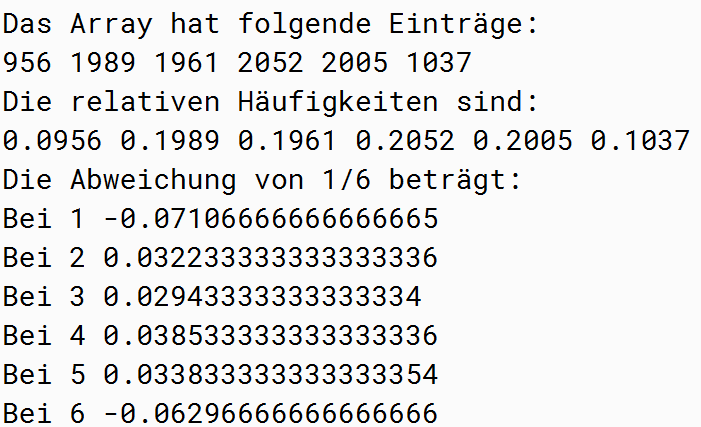
\includegraphics[scale=0.75]{media/schlechte_Ausgabe.png}
\end{center}
Auffallend ist, dass die Zahlen $1$ und $6$ scheinbar deutlich zu selten gewürfelt werden! Sieht man sich unsere Würfel-Methode noch einmal an wird auch klar warum, auf $0$ wird nur von $0$ bis $0,499\dots$ abgerundet und auf $6$ nur von $5,5$ bis $5,99\dots$ aufgerundet, d.h. hier ist der Bereich kleiner, da auf 2 im Bereich von $1,5$ bis $2,499\dots$ gerundet wird. Wir müssen also - wenn wir ganz genau sein wollen - unsere Würfeln-Methode noch anpassen, z.B. so:
\begin{minted}{Java}
    public int würfeln() {
        while(true) {
            int x = (int) Math.round(Math.random()*7);
            if(x != 0 && x != 7) {
                return x;
            }
         }
    }
\end{minted}
Wir erweitern unseren Bereich also, sodass wir von $0$ bis $7$ würfeln können, geben das Ergebnis aber nur zurück, wenn es sich nicht um $0$ oder $7$ handelt. Falls es eine der beiden Zahlen ist, würfeln wir erneut (hier realisiert mit while(true), d.h. es wird so lange ausgeführt, bis einmal das return ausgeführt wird). Neue Ausgabe:
\begin{center}
    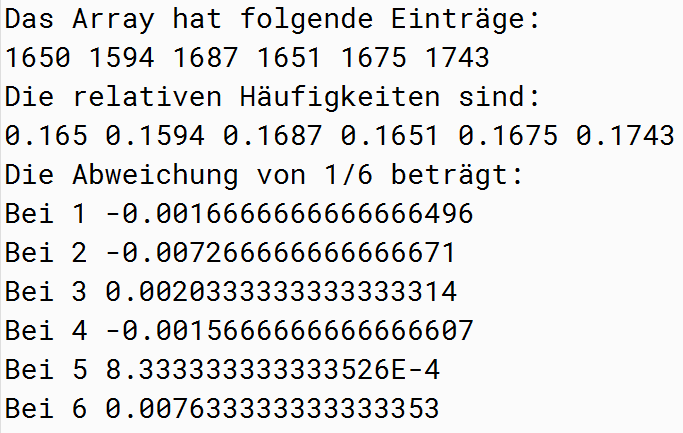
\includegraphics[scale=0.75]{media/bessere_Ausgabe.png}
\end{center}
Besser! $4$ Seiten, es reicht :). Wer durchgehalten hat bis zum Ende: Glückwunsch!
\end{document}